\documentclass[a5paper, 10pt]{article}

% Текст
\usepackage[utf8]{inputenc} % UTF-8 кодировка
\usepackage[russian]{babel} % Русский язык
\usepackage{indentfirst} % красная строка в первом параграфе в главе
% Отображение страниц
\usepackage{geometry} % размеры листа и отступов
\usepackage{listings}
\usepackage{color}

\geometry{
	left=12mm,
	top=25mm,
	right=15mm,
	bottom=17mm,
	marginparsep=0mm,
	marginparwidth=0mm,
	headheight=10mm,
	headsep=7mm,
	nofoot}
\usepackage{afterpage,fancyhdr} % настройка колонтитулов
\pagestyle{fancy}
\fancypagestyle{style}{ % создание нового стиля style
	\fancyhf{} % очистка колонтитулов
	\fancyhead[LO, RE]{Лабораторная работа № 5 } % название документа наверху
	\fancyhead[RO, LE]{Связь непрерывного и дискретного} % название section наверху
	\fancyfoot[RO, LE]{\thepage} % номер страницы справа внизу на нечетных и слева внизу на четных
	\renewcommand{\headrulewidth}{0.25pt} % толщина линии сверху
	\renewcommand{\footrulewidth}{0pt} % толцина линии снизу
}
\fancypagestyle{plain}{ % создание нового стиля plain -- полностью пустого
	\fancyhf{}
	\renewcommand{\headrulewidth}{0pt}
}
\fancypagestyle{title}{ % создание нового стиля title -- для титульной страницы
	\fancyhf{}
	\fancyhead[C]{{\footnotesize
			Министерство образования и науки Российской Федерации\\
			Федеральное государственное автономное образовательное учреждение высшего образования
	}}
	\fancyfoot[C]{{\large 
			Санкт-Петербург, 2024
	}}
	\renewcommand{\headrulewidth}{0pt}
}

% Математика
\usepackage{amsmath, amsfonts, amssymb, amsthm} % Набор пакетов для математических текстов
%\usepackage{dmvnbase} % мехматовский пакет latex-сокращений
\usepackage{cancel} % зачеркивание для сокращений
% Рисунки и фигуры
\usepackage[pdftex]{graphicx} % вставка рисунков
\usepackage{wrapfig, subcaption} % вставка фигур, обтекая текст
\usepackage{caption} % для настройки подписей
\captionsetup{figurewithin=none,labelsep=period, font={small,it}} % настройка подписей к рисункам
% Рисование
\usepackage{tikz} % рисование
\usepackage{circuitikz}
\usepackage{pgfplots} % графики
% Таблицы
\usepackage{multirow} % объединение строк
\usepackage{multicol} % объединение столбцов
% Остальное
\usepackage[unicode, pdftex]{hyperref} % гиперссылки
\usepackage{enumitem} % нормальное оформление списков
\setlist{itemsep=0.15cm,topsep=0.15cm,parsep=1pt} % настройки списков
% Теоремы, леммы, определения...
\theoremstyle{definition}
\newtheorem{Def}{Определение}
\newtheorem*{Axiom}{Аксиома}
\theoremstyle{plain}
\newtheorem{Th}{Теорема}
\newtheorem{Lem}{Лемма}
\newtheorem{Cor}{Следствие}
\newtheorem{Ex}{Пример}
\theoremstyle{remark}
\newtheorem*{Note}{Замечание}
\newtheorem*{Solution}{Решение}
\newtheorem*{Proof}{Доказательство}
% Свои команды
\newcommand{\comb}[1]{\left[\hspace{-4pt}\begin{array}{l}#1\end{array}\right.\hspace{-5pt} } % совокупность уравнений
% Титульный лист
\usepackage{csvsimple-l3}
\newcommand*{\titlePage}{
	\thispagestyle{title}
	\begingroup
	\begin{center}
		%		{\footnotesize
			%			Министерство образования и науки Российской Федерации\\
			%			Федеральное государственное автономное образовательное учреждение высшего образования
			%		}
		%		
		\vspace*{6ex}
		
		{\small
			САНКТ-ПЕТЕРБУРГСКИЙ НАЦИОНАЛЬНЫЙ ИССЛЕДОВАТЕЛЬСКИЙ УНИВЕРСИТЕТ ИТМО	
		}
		
		\vspace*{2ex}
		
		{\normalsize
			Факультет систем управления и робототехники
		}
		
		\vspace*{15ex}
		
		{\Large \bfseries 
			Лабораторная работа № 5
		}
\vspace*{2ex}
	{\Large \bfseries 
			
"Связь непрерывного и дискретного "
		}
\vspace*{2ex}
		
		{\normalsize
			по дисциплине Частотные методы
		}

	\end{center}
	\vspace*{20ex}
	\begin{flushright}
		{\large 
			\underline{Выполнила}: студентка гр. \textbf{R3238}\\
			\begin{flushright}
				\textbf{Нечаева А. А.}\\
			\end{flushright}
		}
		
		\vspace*{5ex}
		
		{\large 
			\underline{Преподаватели}: \textit{Перегудин Алексей Алексеевич,}\\ \textit{Пашенко Артём Витальевич}
		}
	\end{flushright}	
	\newpage
	\setcounter{page}{1}
	\endgroup}

\begin{document}
	\titlePage
	\pagestyle{style}
\newpage



\section{Задание. Непрерывное и дискретное преобразование Фурье.}

Рассмотрим прямоугольную функцию $\Pi : \mathbb{R} \to \mathbb{R}$:

\begin{equation}
\Pi (t) =
\begin{cases}
1, & |t| \leq 1/2,\\
0, & |t| > 1/2
\end{cases}
\end{equation}

\begin{figure}[h!]
\center{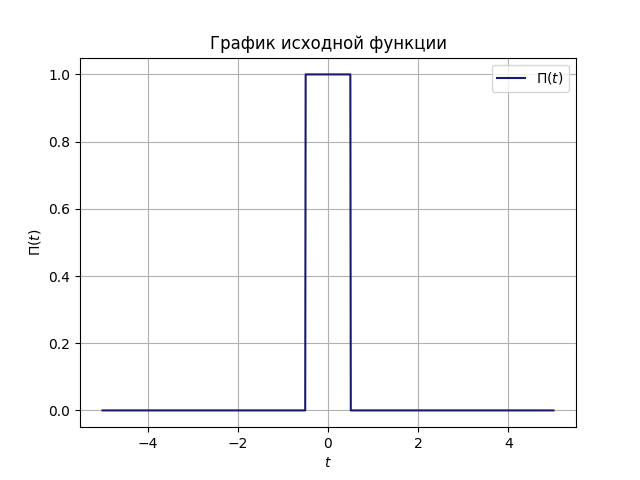
\includegraphics[width=1\linewidth]{pic1/f0.png}}
\caption{График исходной функции $\Pi(t)$.}
\end{figure}

\newpage
\subsection{Истинный Фурье-образ.}
Найдем аналитическое выражение для Фурье-образа

\begin{multline}
\hat{\Pi}(\nu) = \int \limits_{-\infty}^{+\infty} \Pi(t) e^{-2\pi i \nu t} dt = \int \limits_{-0.5}^{0.5} e^{-2\pi i \nu t} dt =
\left. -\frac{e^{-2\pi i \nu t}}{2\pi i \nu} \right|_{-0.5}^{0.5} = \\
= -\frac{e^{-\pi i \nu} - e^{\pi i \nu}}{2\pi i \nu} = \frac{e^{\pi i \nu} - e^{-\pi i \nu}}{2\pi i \nu} = \frac{sin(\pi \nu)}{\pi \nu} = sinc(\nu)
\end{multline}

\begin{figure}[h!]
\center{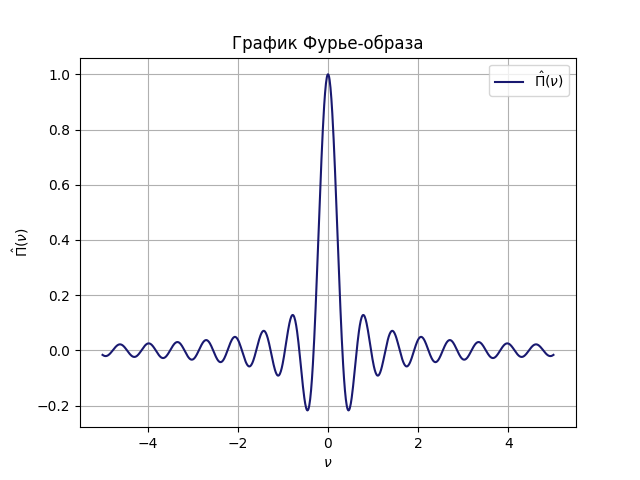
\includegraphics[width=1\linewidth]{pic1/im_0.png}}
\caption{График Фурье-образа функции $\Pi(t)$.}
\end{figure}

\newpage
\subsection{Численное интегрирование}
Теперь найдем Фурье-образ $\Pi(t)$ с помощью численного интегрирования (функции \textit{trapz} библиотеки \textit{NumPy} языка \textit{Python}), а затем с помощью численного интегрирования восстановим исходную функцию $\Pi(t)$.\\

Число шагов интегрирования будем задавать переменной $n$.

\begin{figure}[h!]
\begin{minipage}[h!]{0.5\linewidth}
\center{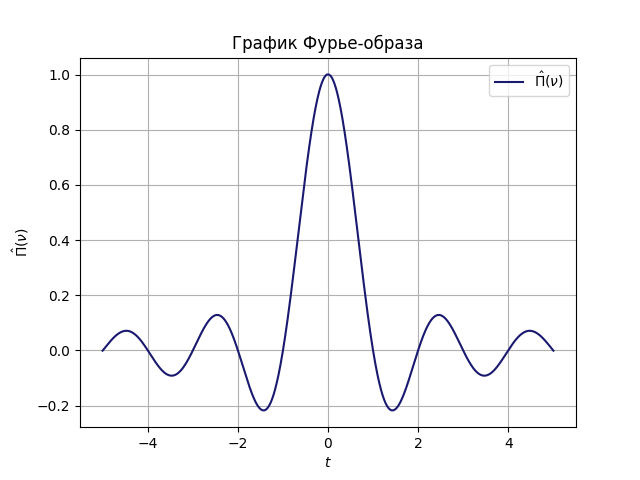
\includegraphics[width=1\linewidth]{pic1/im_c_1}} a) \\
\end{minipage}
\hfill
\begin{minipage}[h!]{0.5\linewidth}
\center{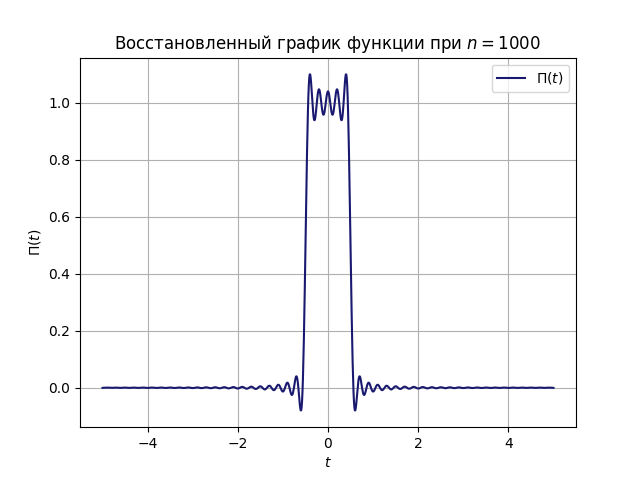
\includegraphics[width=1\linewidth]{pic1/f_re_1}} \\б)
\end{minipage}
\caption{a) График Фурье-образа функции $\Pi(t)$, полученный с помощью численного интегрирования, б) график восстановленной функции.}
\end{figure}

Заметим, что при $n=1000$ график Фурье-образа (рисунок 3а) совпадает с графиком Фурье-образа, построенного с помощью аналитической фомулы (рисунок 2). В то же время, график восстановленной функции (рисунок 3б) имеет заметные отличия от исходного графика функции (рисунок 1). Далее построим сравнительные графики Фурье-образов, исходной функции и восстановленной при разных значениях $n$, также будем фиксировать время работы программы. Промежуток интегрирования обозначим $[-d, d]$.
 Основные характеристики графиков представлены в таблице 1.



\begin{table}[h!]
\caption{Параметры графиков восстановленной функции на промежутке интегрирования $[-5, 5]$.}
\label{tabular:timesandtenses}
\begin{center}
\begin{tabular}{|c|c|c|c|c|c|}
\hline
№ рисунка & объект& $n$ & $d$ & $t, mc$  \\
\hline
 4 а& функция &10000 & 5 &10369  \\
\hline
4 б & образ & 10000 & 5 & 5341 \\
\hline
5 а &  функция &200  & 5 & 196 \\
\hline
5 б & образ & 200  & 5  & 202 \\
\hline
5 в &  функция & 100  & 5  & 198 \\
\hline
5 г & образ & 100  & 5  & 276 \\
\hline
6 а &  функция & 90  & 5  & 270 \\
\hline
6 б & образ & 90  & 5  & 236 \\
\hline
\end{tabular}
\end{center}
\end{table}



\begin{figure}[h!]
\begin{minipage}[h!]{0.5\linewidth}
\center{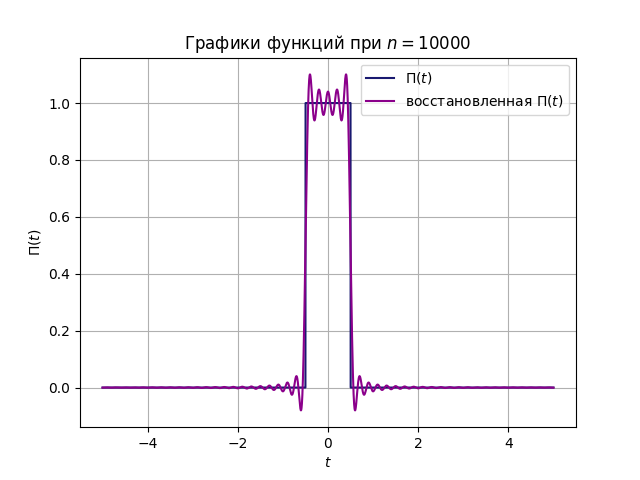
\includegraphics[width=1\linewidth]{pic1/f_n_10000_5.png}} a) \\
\end{minipage}
\hfill
\begin{minipage}[h!]{0.5\linewidth}
\center{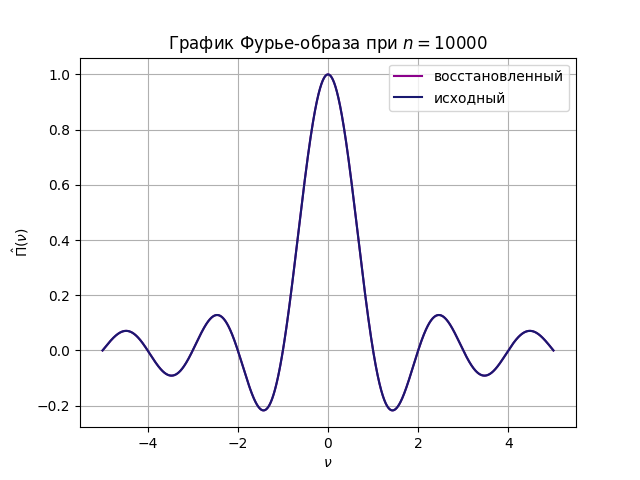
\includegraphics[width=1\linewidth]{pic1/im_n_10000_5.png}} \\б)
\end{minipage}
\caption{ Графики восстановленной и исходной функции и их Фурье-образов при $n=10000$.}
\end{figure}

\begin{figure}[h!]
\begin{minipage}[h!]{0.5\linewidth}
\center{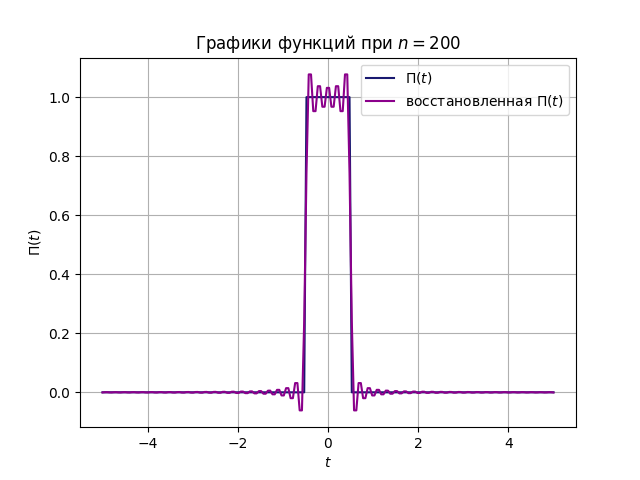
\includegraphics[width=1\linewidth]{pic1/f_n_200_5.png}} \\а)
\end{minipage}
\hfill
\begin{minipage}[h!]{0.5\linewidth}
\center{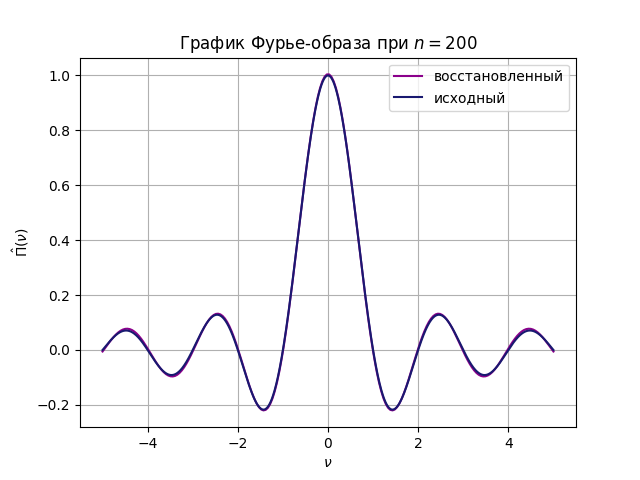
\includegraphics[width=1\linewidth]{pic1/im_n_200_5.png}} \\б)
\end{minipage}
\vfill
\begin{minipage}[h!]{0.5\linewidth}
\center{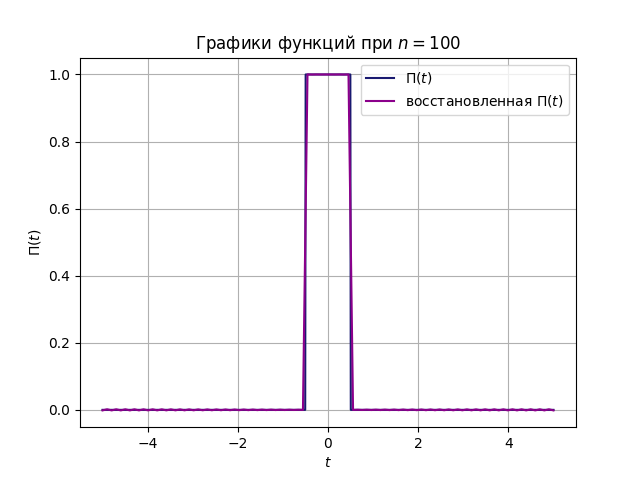
\includegraphics[width=1\linewidth]{pic1/f_n_100_5.png}} \\в)
\end{minipage}
\hfill
\begin{minipage}[h!]{0.5\linewidth}
\center{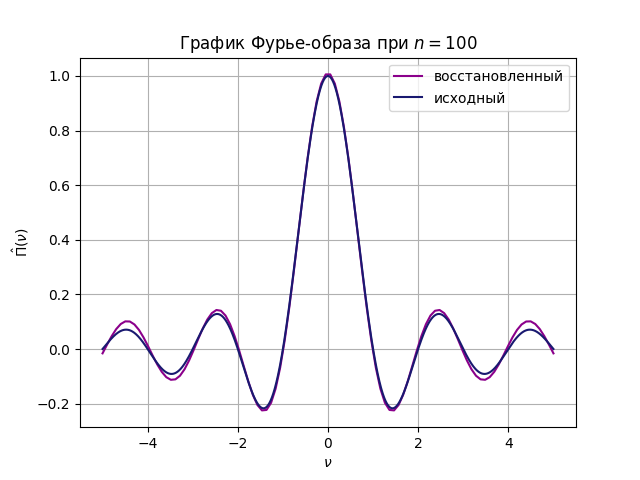
\includegraphics[width=1\linewidth]{pic1/im_n_100_5.png}} \\г)
\end{minipage}
\caption{ Графики восстановленной и исходной функции и их Фурье-образов при $n=200, \, 100$.}
\end{figure}

\begin{figure}[h!]
\begin{minipage}[h!]{0.5\linewidth}
\center{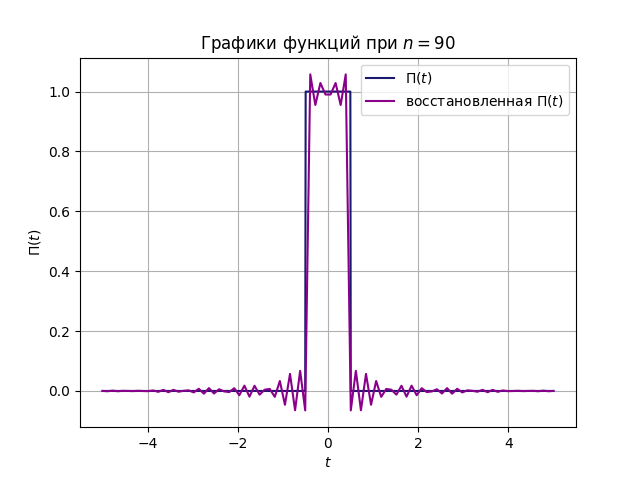
\includegraphics[width=1\linewidth]{pic1/f_n_90_5.png}} a) \\
\end{minipage}
\hfill
\begin{minipage}[h!]{0.5\linewidth}
\center{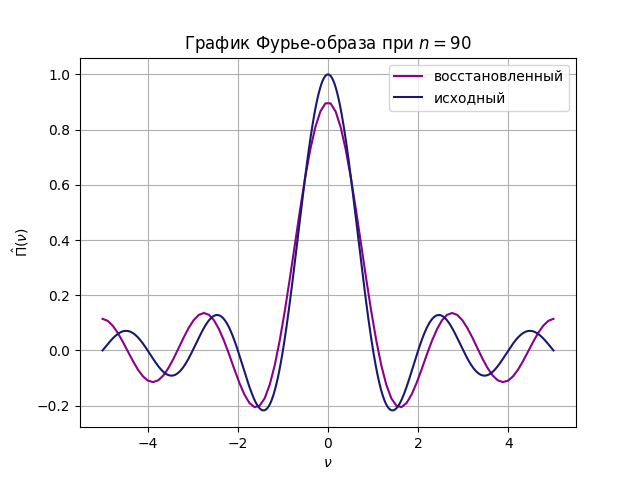
\includegraphics[width=1\linewidth]{pic1/im_n_90_5.png}} \\б)
\end{minipage}
\caption{ Графики восстановленной и исходной функции и их Фурье-образов при $n=90$.}
\end{figure}


\newpage

Сравнивая графики на рисунках 4 а, 5 а, 5 в, можно сделать вывод о том, что при уменьшении числа итераций в вычислении интегралов для нахождения Фурье-образа и последующего восстановления функции, сходство графиков исходной и восстановленной функций возрастает.\\

 Однако при дальнейшем уменьшении $n$ $(n < 100)$ различия между графиками исходной и восстановленной функций возрастают (рисунки 5в и 5г). Время выполнения также возрастает (таблица 1).\\

Наиболее оптимальным по результату и времени выполнения в нашем случае является $n=100$.

\begin{table}[h!]
\caption{Параметры графиков восстановленной функции на промежутке интегрирования $[-1, 1]$.}
\label{tabular:timesandtenses}
\begin{center}
\begin{tabular}{|c|c|c|c|c|c|}
\hline
№ рисунка & объект & $n$ & $d$ & $t, mc$  \\
\hline
 7 а&  функция &1000 & 1 & 486 \\
\hline
 7 б& образ & 1000 & 1 & 287 \\
\hline
8 а  & функция & 30 & 1 & 241 \\
\hline
8 б & образ & 30  & 1 &  211\\
\hline
8 в & функция & 10  & 1  & 191 \\
\hline
8 г & образ & 10  & 1  & 274 \\
\hline
9 а & функция & 5  & 1  & 161 \\
\hline
9 б & образ & 5  & 1  & 188 \\
\hline
\end{tabular}
\end{center}
\end{table}



\begin{figure}[h!]
\begin{minipage}[h!]{0.5\linewidth}
\center{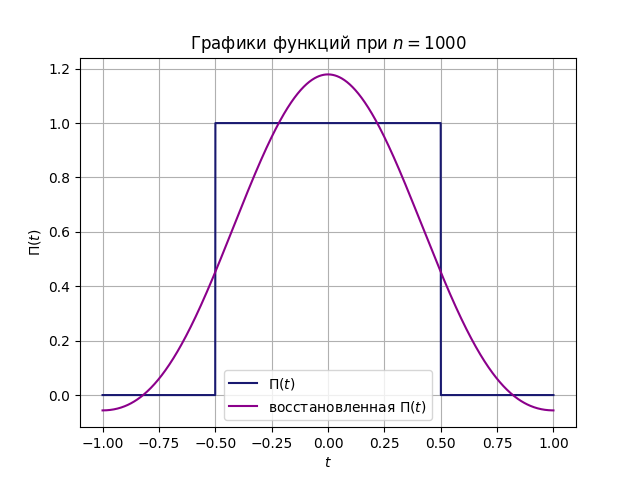
\includegraphics[width=1\linewidth]{pic1/f_n_1000_1.png}} \\а)
\end{minipage}
\hfill
\begin{minipage}[h!]{0.5\linewidth}
\center{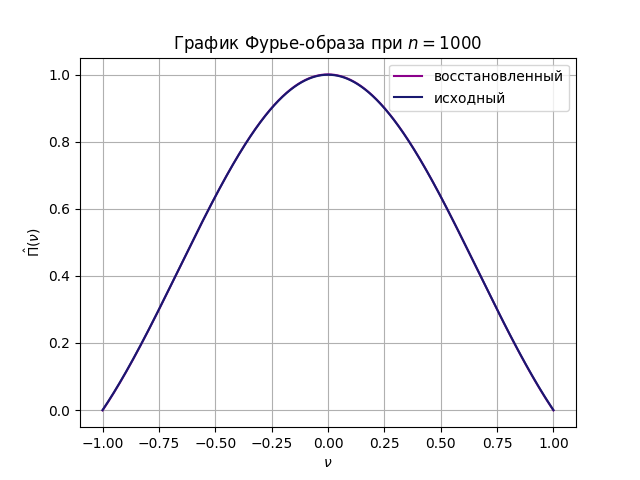
\includegraphics[width=1\linewidth]{pic1/im_n_1000_1.png}} \\б)
\end{minipage}
\caption{ Графики восстановленной и исходной функции и их Фурье-образов при $n=1000$.}
\end{figure}

\begin{figure}[h!]
\begin{minipage}[h!]{0.5\linewidth}
\center{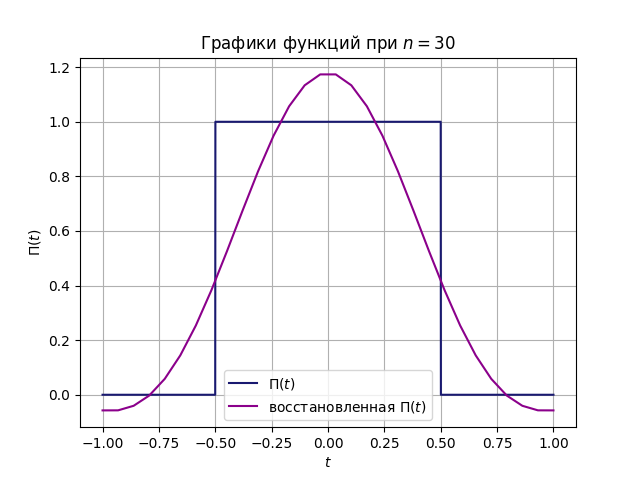
\includegraphics[width=1\linewidth]{pic1/f_n_30_1.png}} \\а)
\end{minipage}
\hfill
\begin{minipage}[h!]{0.5\linewidth}
\center{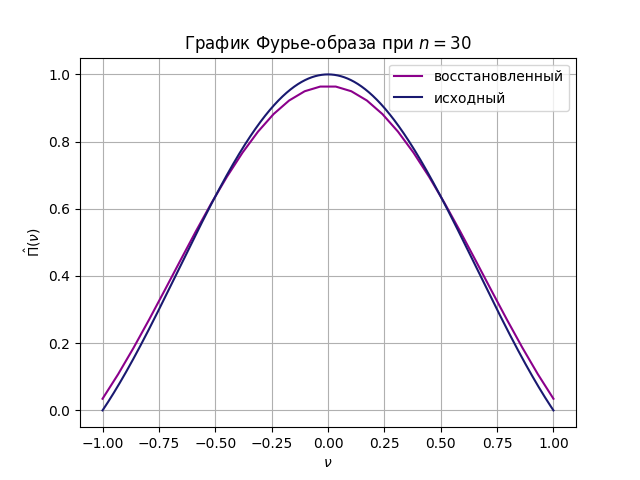
\includegraphics[width=1\linewidth]{pic1/im_n_30_1.png}} \\б)
\end{minipage}
\vfill
\begin{minipage}[h!]{0.5\linewidth}
\center{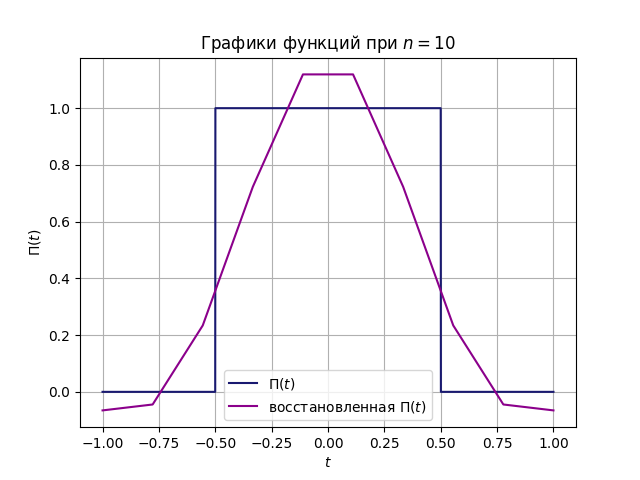
\includegraphics[width=1\linewidth]{pic1/f_n_10_1.png}} \\в)
\end{minipage}
\hfill
\begin{minipage}[h!]{0.5\linewidth}
\center{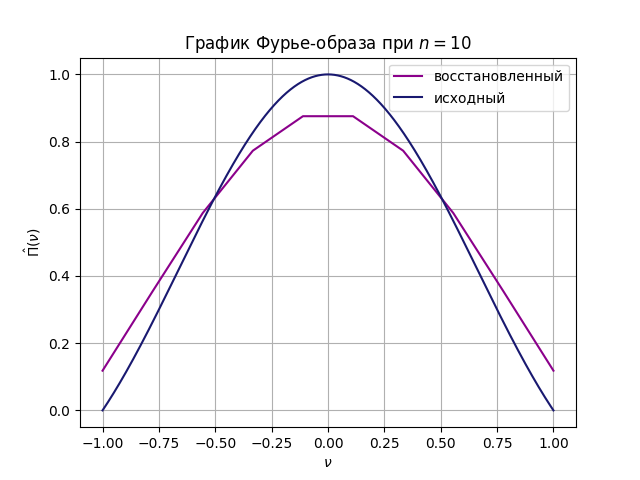
\includegraphics[width=1\linewidth]{pic1/im_n_10_1.png}} \\г)
\end{minipage}
\caption{ Графики восстановленной и исходной функции и их Фурье-образов при $n=30, \, 10$.}
\end{figure}

\begin{figure}[h!]
\begin{minipage}[h!]{0.5\linewidth}
\center{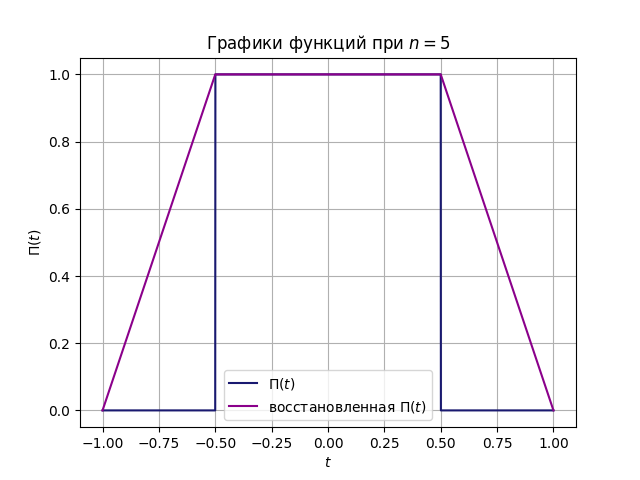
\includegraphics[width=1\linewidth]{pic1/f_n_5_1.png}} \\а)
\end{minipage}
\hfill
\begin{minipage}[h!]{0.5\linewidth}
\center{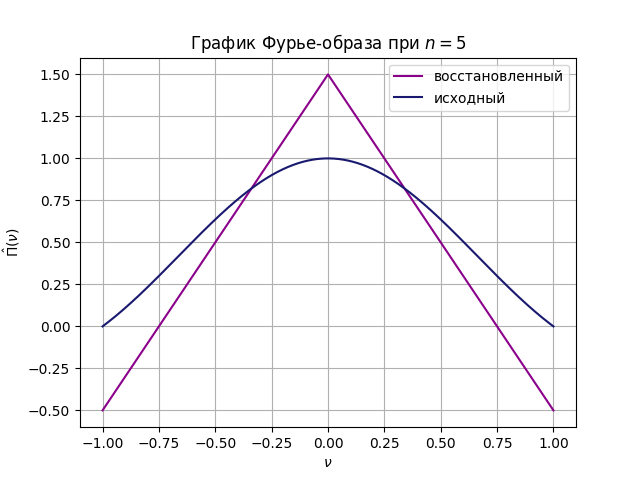
\includegraphics[width=1\linewidth]{pic1/im_n_5_1.png}} \\б)
\end{minipage}
\caption{ Графики восстановленной и исходной функции и их Фурье-образов при $n=5$.}
\end{figure}


\newpage
\,
\newpage
Заметим, что при $n=1000$ и при $n=30$ существенной разницы между восстановленными функциями нет (рисунок 7 а и 8 а), кроме того, что в восстановаленной функции на рисунке 8 а отчетливее видны ломанная, из которой она состоит. При дельнейшем уменьшении $n$ точность восстановленной функции снижается. Время работы программы также снижается и достигает минимума при $n=5$, далее опять увеличивается.\\

 Наиболее оптимальными с точки зрения точности приближения исходного графика функции и времени выполнения в данном случае являются $n=5$ и $n=6$.\\


Теперь рассмотрим интегрирование на промежутке $[-10, 10]$, то есть при $d=10$.





\begin{table}[h!]
\caption{Параметры графиков восстановленной функции на промежутке интегрирования $[-10, 10]$.}
\label{tabular:timesandtenses}
\begin{center}
\begin{tabular}{|c|c|c|c|c|c|}
\hline
№ рисунка & объект & $n$ & $d$ & $t, mc$  \\
\hline
 10 а&  функция &10000 & 10 &  10766\\
\hline
 10 б& образ & 10000 & 10 & 5302 \\
\hline
10 в  & функция & 1000 & 10 & 390 \\
\hline
10 г & образ & 1000  & 10 & 281 \\
\hline
11 а  &  функция &500 & 10 & 271 \\
\hline
11 б &образ & 500  & 10 & 192 \\
\hline
11 в & функция & 250  & 10 & 223 \\
\hline
11 г & образ & 250  & 10  &  188 \\
\hline
\end{tabular}
\end{center}
\end{table}



\begin{figure}[h!]
\begin{minipage}[h!]{0.5\linewidth}
\center{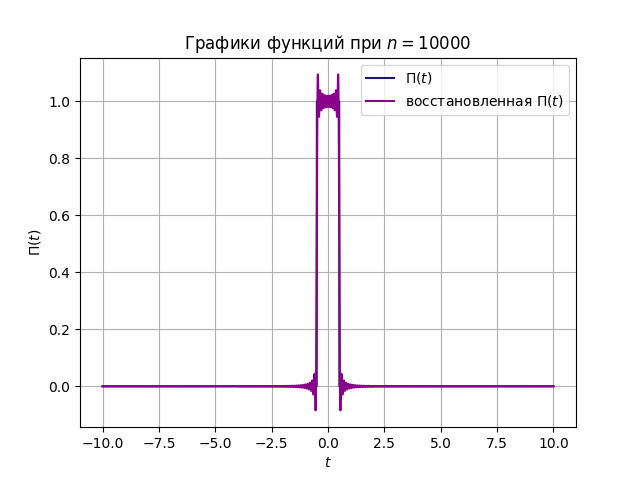
\includegraphics[width=1\linewidth]{pic1/f_n_10000_10.png}} \\а)
\end{minipage}
\hfill
\begin{minipage}[h!]{0.5\linewidth}
\center{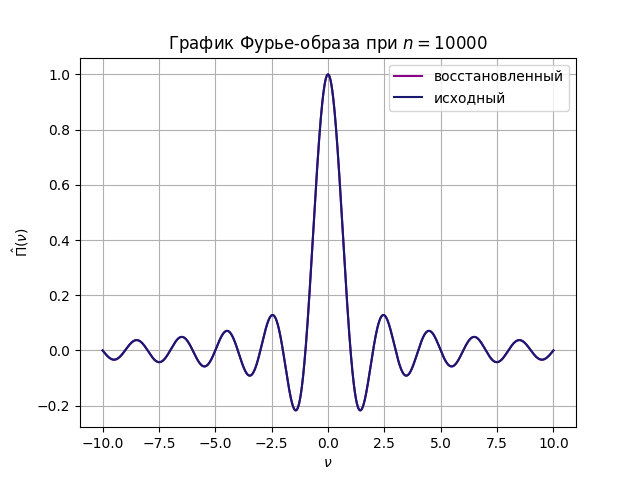
\includegraphics[width=1\linewidth]{pic1/im_n_10000_10.png}} \\б)
\end{minipage}
\vfill
\begin{minipage}[h!]{0.5\linewidth}
\center{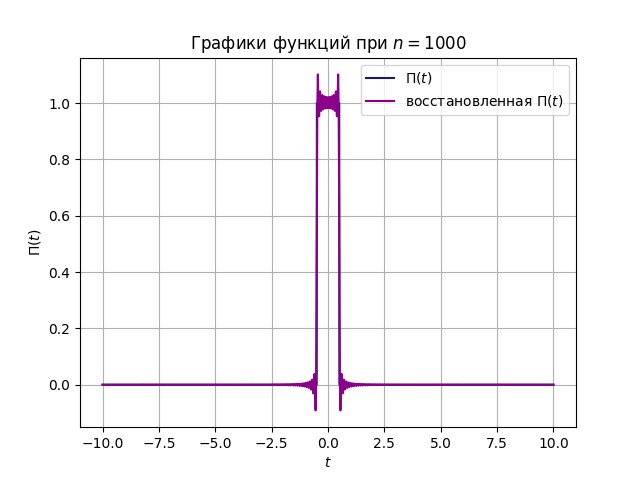
\includegraphics[width=1\linewidth]{pic1/f_n_1000_10.png}} \\в)
\end{minipage}
\hfill
\begin{minipage}[h!]{0.5\linewidth}
\center{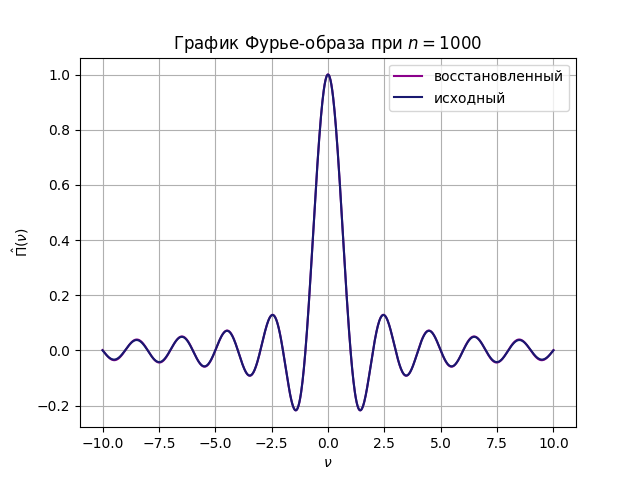
\includegraphics[width=1\linewidth]{pic1/im_n_1000_10.png}} \\г)
\end{minipage}
\caption{ Графики восстановленной и исходной функции и их Фурье-образов при $n=10000, \, 1000$.}
\end{figure}

\newpage
Заметим, что при $n=10000$ и $n=1000$ для случая $d=10$ результат на графике практически идентичен, но время, затраченное на вычисление последнего примерно в 30 раз меньше. С точки зрения точности приближения в обоих случаях график исходной функции узнаваем, наибольшие различия замечены в точках скачков функции.\\




\begin{figure}[h!]
\vfill
\begin{minipage}[h!]{0.5\linewidth}
\center{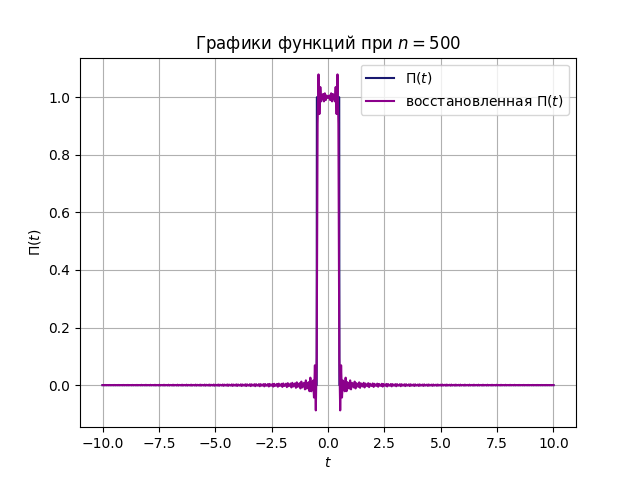
\includegraphics[width=1\linewidth]{pic1/f_n_500_10.png}} \\а)
\end{minipage}
\hfill
\begin{minipage}[h!]{0.5\linewidth}
\center{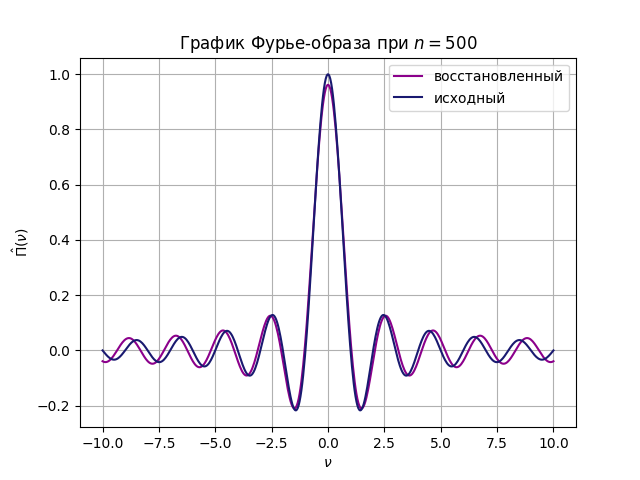
\includegraphics[width=1\linewidth]{pic1/im_n_500_10.png}} \\б)
\end{minipage}
\vfill
\begin{minipage}[h!]{0.5\linewidth}
\center{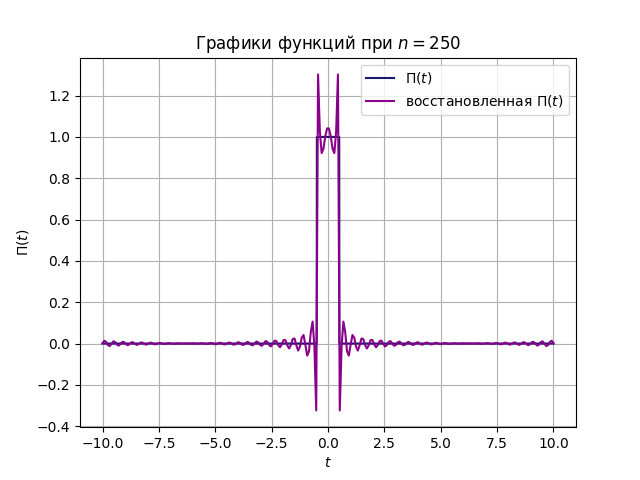
\includegraphics[width=1\linewidth]{pic1/f_n_250_10.png}} \\в)
\end{minipage}
\hfill
\begin{minipage}[h!]{0.5\linewidth}
\center{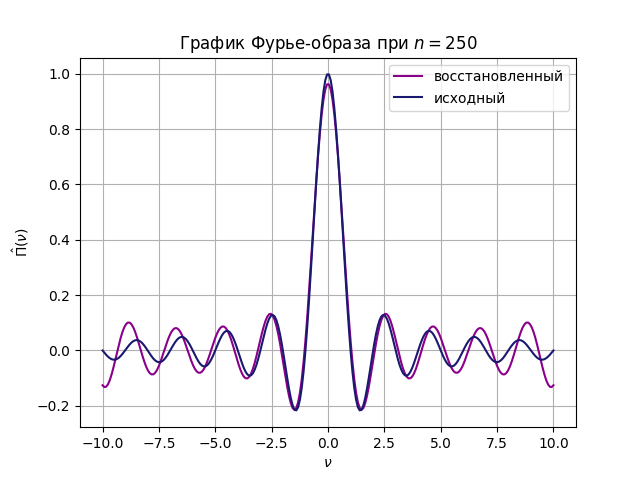
\includegraphics[width=1\linewidth]{pic1/im_n_250_10.png}} \\г)
\end{minipage}
\caption{ Графики восстановленной и исходной функции и их Фурье-образов при $n=500, \, 250$.}
\end{figure}


\newpage
При $n=500$ получаем еще удовлетворительный результат: исходная функция угадывается по графику восстановленной, в ходе дальнейшего уменьшении $n < 500$ график восстановленной функции все меньше похож на исходную.\\


\newpage
\,
\newpage
\textbf{Вывод.} Для получения оптимального результата требуется достаточно большое количество времени: $200-300$ мс. Точность позволяет узнать в восстановленной функции исходную, пусть и с небольшими помехами в областях скачков функции. 












\newpage
\subsection{Использование DFT}
Найдем Фурье-образ функции $\Pi (t)$ с помощью дискретного преобразования Фурье (конструкция \textit{fftshift(fft())}), используя его так, чтобы преобразование было \textit{унитарным}. Затем выполним обратное преобразование от найденного Фурье-образа с помощью обратного дискретного преобразования. Сначала запишем, как работают преобразования:
$$numpy.fft.fft:$$
\begin{equation}
y(j) = \sum \limits_{k=0}^{n-1} x(k) \cdot \exp \left\{ - \frac{2\pi  i j k}{n} \right\}
\end{equation}

$$numpy.fft.ifft:$$

\begin{equation}
x(k) = \frac{1}{n} \sum \limits_{j=0}^{n-1} y(j) \cdot \exp \left\{ \frac{2\pi  i j k}{n} \right\}
\end{equation}
Для того, чтобы преобразования стали \textit{унитарными}:  $$F(j) = \frac{ y(j)}{\sqrt{n}} , \, \, \, \, \, \, \, \, \, \, f(k) = x(k)\sqrt{n}.$$


\begin{table}[h!]
\caption{Параметры графиков восстановленной с помощью DFT функции и ее Фурье-образа на промежутке интегрирования $[-5, 5]$.}
\label{tabular:timesandtenses}
\begin{center}
\begin{tabular}{|c|c|c|c|c|c|}
\hline
№ рисунка & объект& $n$ & $d$ & $t, mc$  \\
\hline
 12 а& функция & 10000 & 5 &  174\\
\hline
 12 б& образ & 10000 & 5& 174 \\
\hline
\end{tabular}
\end{center}
\end{table}

Заметим, что относительно аналогичного случая применения \textit{trapz}, то есть при $n = 10000$ и $d = 5$, скорость выполнения с помощью DFT возрасла примерно в 100 раз, для сравнения для получения восстановленной функции с помощью численного интегрирования понадобилось \textbf{10369} мс, а для DFT \textbf{174} мс. График восстановленной функции визуально совпадает с графиком исходной, но Фурье-образ, полученный с помощью DFT сильно отличается от графика истинного Фурье-образа, хотя при использовании численного интегрирования (рисунок 4б) Фурье-образы восстановленной и исходной функций совпадают.


\begin{figure}[h!]
\begin{minipage}[h!]{0.5\linewidth}
\center{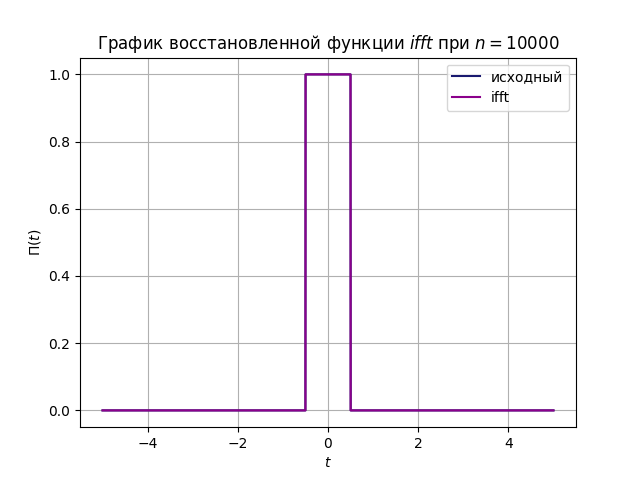
\includegraphics[width=1\linewidth]{pic1/fft_f.png}} \\а)
\end{minipage}
\hfill
\begin{minipage}[h!]{0.5\linewidth}
\center{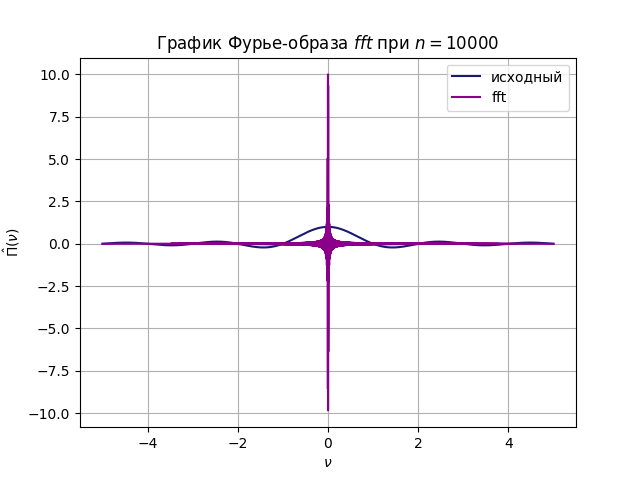
\includegraphics[width=1\linewidth]{pic1/fft_im.png}} \\б)
\end{minipage}
\caption{ Графики восстановленной и исходной функции и их Фурье-образов при $n=10000$.}
\end{figure}

\subsection{Объяснения}

\subsubsection{ Быстрота выполнения с помощью DFT.}
Скорость DFT объясняется алгоритмамми, которые работают "под капотом" функций из библиотеки \textit{NumPy}. Алгоритмы используют свойство симметрии, например, рассмотрим вычисление следующего компонента Фурье-образа:
\begin{multline}
y(j + n) = \sum \limits_{k=0}^{n-1} x(k) \cdot \exp \left\{ - \frac{2\pi  i (n + j) k}{n} \right\} =  \sum \limits_{k=0}^{n-1} x(k) \cdot \exp \left\{ - 2\pi  i  k \right\} \cdot \exp \left\{ - \frac{2\pi  i  j k}{n} \right\} =\\= \sum \limits_{k=0}^{n-1} x(k) \cdot \exp \left\{ - \frac{2\pi  i  j k}{n} \right\} = y(j)
\end{multline}

Заметим свойство симметрии: $y(j + z \cdot n) = y(j)$, где $z \in \mathbb{Z}$.\\

 Последовательно применяя этот инструмент, рекурсивно постоянно разделяя массив, который необходимо вычислить, добиваемся того, что ассимптотика алгоритма становится $O(n \log n)$ вместо $O(n^2)$, которая получается при преобразовании Фурье без использования оптимизации.


\newpage
\subsubsection{Отличие образа после DFT.}

Предположим, что различия вызваны несоответствием дискретной формулы, использованной в DFT, непрерывной фурмуле для нахождения Фурье-образа. Запишем аналитическое выражение для Фурье-образа

\begin{equation}
\hat{\Pi}(\nu) = \int \limits_{-\infty}^{+\infty} \Pi(t) e^{-2\pi i \nu t} dt
\end{equation}
И попробуем от непрерывного интеграла перейти к дискретной сумме. 
\begin{multline}
\hat{\Pi}(\nu) = \int \limits_{-\infty}^{+\infty} \Pi(t) e^{-2\pi i \nu t} dt \sim \sum \limits_{k=0}^{n-1} \Pi(t_0 + k \cdot \Delta t)  \exp \left\{ - 2\pi  i \nu (t_0 + k \cdot \Delta t) \right\} \Delta t = \\ = e^{ - 2\pi  i \nu t_0 } \Delta t  \sum \limits_{k=0}^{n-1} \Pi(t_0 + k \cdot \Delta t)  e^{ - 2\pi  i \nu  k \cdot \Delta t}
\end{multline}
Пусть $\widetilde{\nu} = m \Delta \nu $ -- дискретная частота, $\widetilde{t} = t_0 + k \Delta t$ -- дискретное время.

\begin{multline}
\hat{\Pi}(\widetilde{\nu}) = e^{ - 2\pi  i \widetilde{\nu} t_0} \Delta t  \sum \limits_{k=0}^{n-1} \Pi(t_0 + k \cdot \Delta t)  e^{ - 2\pi  i \Delta \nu  k \cdot \Delta t}= \\ = e^{ - 2\pi  i \widetilde{\nu} t_0} \Delta t  \sum \limits_{k=0}^{n-1} \Pi(\widetilde{t})  \exp \left\{ - \frac{2\pi  i  m \cdot k}{n} \right\}
\end{multline}

Заметим, что полученное выражение похоже на формулу для Фурье-образа DFT с точностью до множителя перед знаком сумматора.




\subsection{Приближение непрерывного с помощью DFT}
Запишем формулу для приближения непрерывного с помощью унитарного DFT -- умное использование fft:

\begin{equation}
\hat{\Pi}(\widetilde{\nu}) = \frac{\Delta t }{\sqrt{n}} e^{ - 2\pi  i \widetilde{\nu} t_0}  \sum \limits_{k=0}^{n-1} \Pi(\widetilde{t})  \exp \left\{ - \frac{2\pi  i  m \cdot k}{n} \right\}
\end{equation}

Теперь запишем умное использование ifft:
\begin{equation}
\Pi (\widetilde{t}) = \frac{\Delta \nu }{\sqrt{n}}   \sum \limits_{m=0}^{n-1} \Pi(\widetilde{\nu})  \exp \left\{  \frac{2\pi  i  k \cdot m}{n} \right\} 
\end{equation}

\begin{figure}[h!]
\center{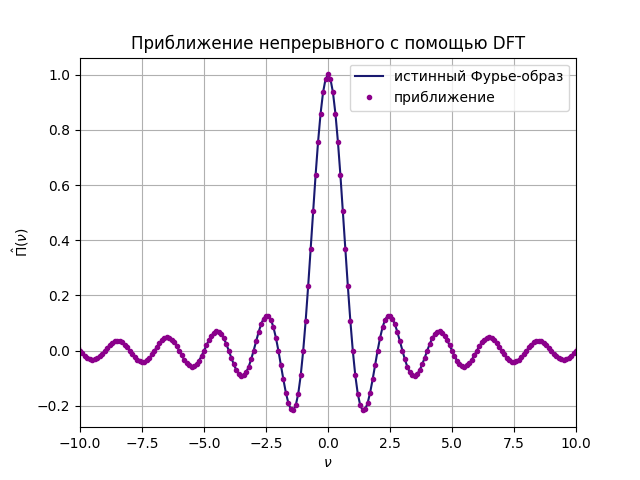
\includegraphics[width=0.77\linewidth]{pic1/DFT_cor.png}}
\caption{Графики истинного и Фурье-образа, полученного с помощью умного fft.}
\center{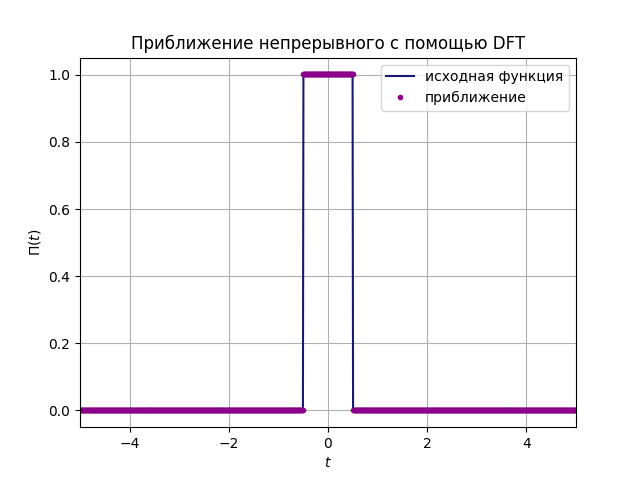
\includegraphics[width=0.77\linewidth]{pic1/cor_fun.png}}
\caption{Графики исходной и функции, полученной с помощью умного ifft.}
\end{figure}




\newpage
\section{Задание. Сэмплирование.}

\subsection{Сэмплирование синусов}
Зададимся параметрами $a_1=1$, $a_2=2$, $\omega_1 = 3$, $\omega_2 = 4$, $\phi_1 = \pi$, $\phi_2 = 2\pi$ и рассмотрим функцию $y(t) = a_1 \sin \left( \omega_1 t + \phi_1 \right) + a_2 \sin \left(  \omega_2 t + \phi_2 \right)$

\begin{equation}
y(t) =  \sin \left( 3 t + \pi \right) + 2 \sin \left(  4 t + 2\pi \right)
\end{equation}

\subsubsection{Построение непрерывного графика}
\begin{figure}[h!]
\center{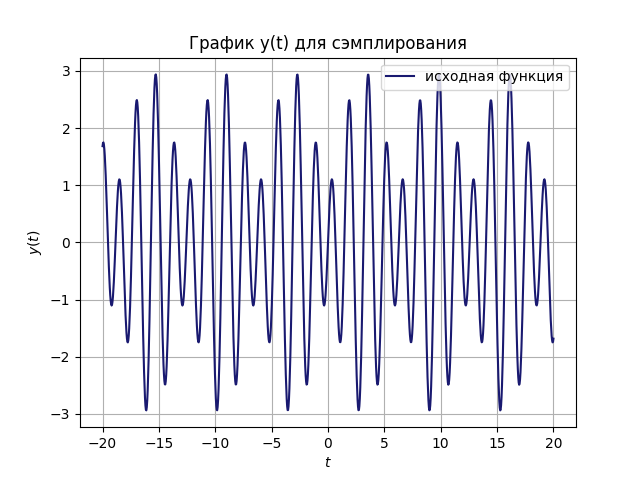
\includegraphics[width=1\linewidth]{pic2/fsin.png}}
\caption{График исходной функции $y(t)$.}
\end{figure}

\subsubsection{Сэмплированный вариант функции}

Рассмотрим разреженный вариант массива времени и соответствующий ему массив значений.
\begin{figure}[h!]
\center{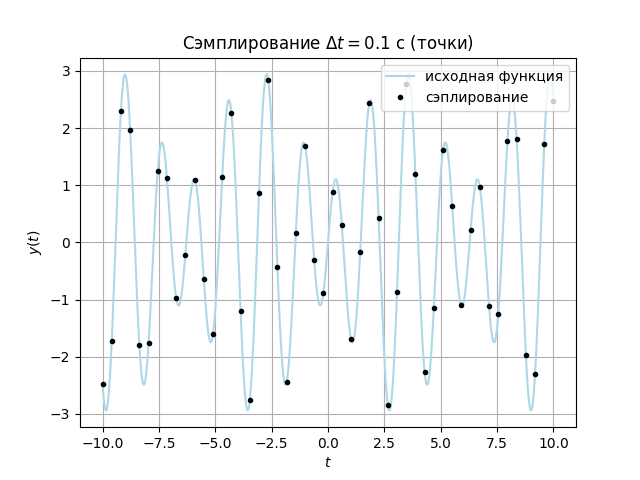
\includegraphics[width=0.77\linewidth]{pic2/s_sample_p.png}}
\caption{Исходный и график после сэмплирования (точки).}
\center{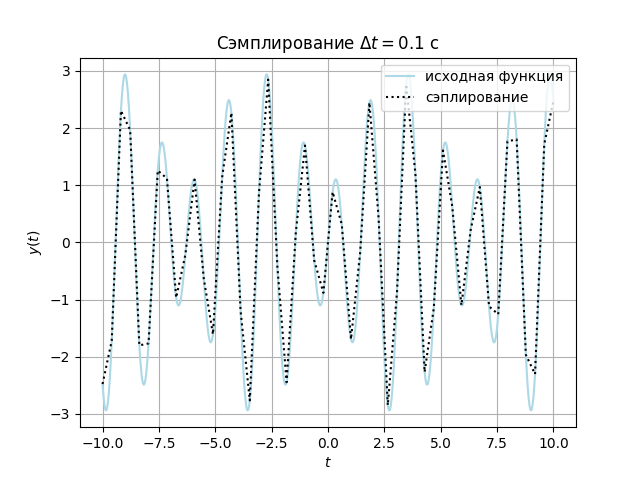
\includegraphics[width=0.77\linewidth]{pic2/s_sample_c.png}}
\caption{Исходный и график после сэмплирования.}
\end{figure}

\subsubsection{Восстановление функции}
Применим интерполяционную формулу $f(t) = \sum \limits_{-\infty}^{\infty} f \left( t_n \right) sinc \left(2Bt - t_n \right)$ к сэмплированным данным с целью восстановления непрерывной функции.

\begin{figure}[h!]
\center{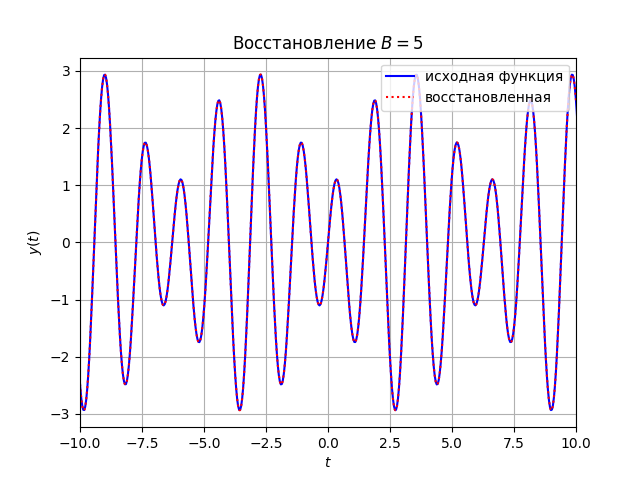
\includegraphics[width=1\linewidth]{pic2/restore_sin.png}}
\caption{Исходный график функции и восстановленный после сэмплирования.}
\end{figure}

\subsubsection{Влияние шага дискретизации}


\subsection{Сэмплирование sinus cardinalis}
\textit{...В работе...}

\end{document}













